\documentclass{article}
\usepackage[T1]{fontenc}
\usepackage[utf8]{inputenc}
\usepackage{hyperref}
\usepackage{lmodern}
\usepackage{gensymb}
\usepackage{minted}
\usepackage{graphicx}
\usepackage{xcolor}
\usepackage{chemfig}
\usepackage{tcolorbox}
\usepackage{amsthm}
\usepackage{subcaption}
\newcommand\aug{\fboxsep=-\fboxrule\!\!\!\fbox{\strut}\!\!\!}
\usepackage{physics}\definecolor{monokaibg}{HTML}{272822}
\definecolor{friendlybg}{HTML}{f0f0f0}
\usepackage[utf8]{inputenc}
\usepackage{amsmath}

\usepackage{listings}
\lstset{language=C++,
    keywordstyle=\color{blue}\bfseries,
    commentstyle=\color{green},
    stringstyle=\ttfamily\color{red!50!brown},
    showstringspaces=false}
\lstset{literate=%
   *{0}{{{\color{red!20!violet}0}}}1
    {1}{{{\color{red!20!violet}1}}}1
    {2}{{{\color{red!20!violet}2}}}1
    {3}{{{\color{red!20!violet}3}}}1
    {4}{{{\color{red!20!violet}4}}}1
    {5}{{{\color{red!20!violet}5}}}1
    {6}{{{\color{red!20!violet}6}}}1
    {7}{{{\color{red!20!violet}7}}}1
    {8}{{{\color{red!20!violet}8}}}1
    {9}{{{\color{red!20!violet}9}}}1
}
\definecolor{codegreen}{rgb}{0,0.6,0}
\definecolor{codegray}{rgb}{0.5,0.5,0.5}
\definecolor{codepurple}{rgb}{0.58,0,0.82}
\definecolor{backcolour}{rgb}{0.95,0.95,0.92}
\lstdefinestyle{mystyle}{
    backgroundcolor=\color{backcolour},   
    commentstyle=\color{codegreen},
    keywordstyle=\color{magenta},
    numberstyle=\tiny\color{codegray},
    stringstyle=\color{codepurple},
    basicstyle=\ttfamily\footnotesize,
    breakatwhitespace=false,         
    breaklines=true,                 
    captionpos=b,                    
    keepspaces=true,                 
    numbers=left,                    
    numbersep=5pt,                  
    showspaces=false,                
    showstringspaces=false,
    showtabs=false,                  
    tabsize=2
}
\lstset{style=mystyle}






\usepackage{xcolor}
\renewcommand{\arraystretch}{1.5}
\setlength\arraycolsep{10pt}  
\newcommand{\uvec}[1]{\boldsymbol{\hat{\textbf{#1}}}}
\newcommand\sbullet[1][.5]{\mathbin{\vcenter{\hbox{\scalebox{#1}{$\bullet$}}}}}







\title{\Huge{ PROJECT 1 }}
\author{Computational Physics - FYS3150}
\date{\today}

\begin{document}
\maketitle
\centerline{Duncan Wilkins | Fuad Dadvar | Don Phillip Bullecer | Erling Nupen}
\centerline{https://github.com/dondondooooon/FYS3150}
\subsection*{Introduction}
The overall topic of this project is numerical solution of the one-dimensional Poisson equation. This is a second-order differential equation that shows up in several areas of physics, e.g. electrostatics. In future projects we will pay close attention to scaling of dimensional physics equations, but for this first project we start directly from the differential equation after scaling to dimensionless variables
\vskip 0.01in
\begin{flushleft}
The one-dimensional Poisson equation can be written as

\end{flushleft}
\begin{equation}\label{likn.1}
    -\frac{d^2u}{dx^2} = f(x)
\end{equation}
Here $f(x)$ is a known function (the source term). Our task is to find the function $u(x)$ that satisfies this equation for a given boundary condition. The specific setup we will assume is the following:
\vskip 0.1in
$\sbullet[.75]\hspace{0.2cm}$ source term: $f(x) = 100e^{-10x}$
\vskip 0.1in
$\sbullet[.75]\hspace{0.2cm}$ $x$ range: $x\in [0,1]$
\vskip0.1in
$\sbullet[.75]\hspace{0.2cm}$ boundry condition: u(0)=0, u(1) = 0
\subsection*{Problem I}
In this task we're to check if that an exact solution to equation(\ref{likn.1}) is given by
\begin{equation}\label{likn.2}
    u(x) = 1 - (1-e^{-10})x-e^{-10x}
\end{equation}
If $u(x)$ is a solution to equation (1) in the problem text, then the following relation must hold:
\begin{equation}\label{likn3}
    \frac{d^2}{dx^2}((1-(1-e^{-10})x - e^{-10x})) = -100e^{-10x} = f(x)
\end{equation}
Its quite straight forward to differentiate $u(x)$. Since it is a second order derivative, all first order terms of $x$ will not survive the derivation. So we end up with $u''(x) = - 10 \cdot (-10)(-10) e^{-10x}$ which is exactly equal to $f(x)$ and therefore is a solution to our equation.

\subsection*{Problem II}
\begin{flushleft}
We wrote a program in C++ shown in   that evaluates equation(\ref{likn.2})
which is the exact solution u(x) for a given array of x values of length 
N = 1000.
\vskip 0.01in
The program generates a data text file, and we use a short plotting script 
such as in Listing(\ref{lst2}) in python to read our data file and generate the plot shown under in figur(\ref{figur1})
\end{flushleft}
\begin{figure}[h]
    \centering %Centers the figure
    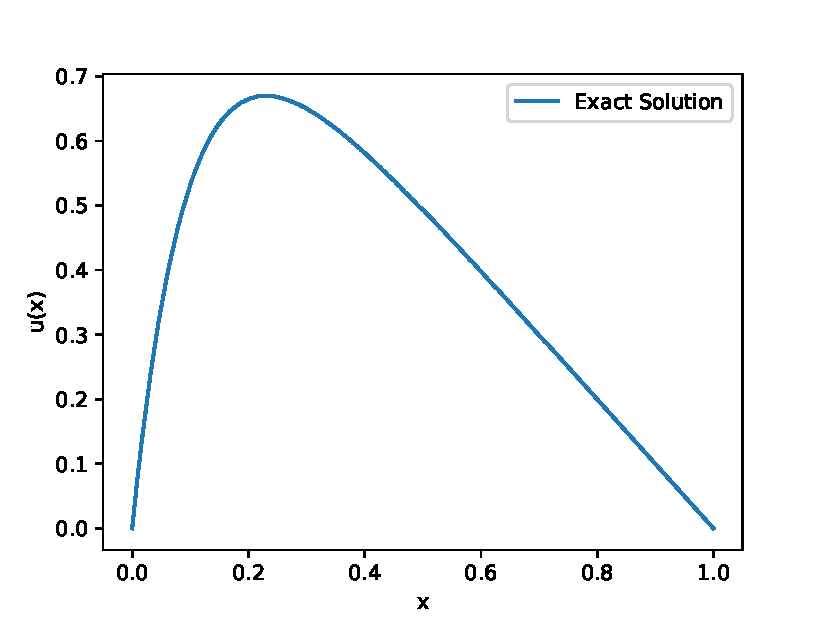
\includegraphics[scale=0.55]{Problem2/Exact_Solution_plot.pdf} %Imports the figure.
    \caption{Plot of x vs. u(x)}
    \label{figur1}
\end{figure}
\pagebreak

\lstinputlisting[label=lst1,language=C++]{Problem2/prob2.cpp}
\begin{lstlisting}[language=C++, label=lst2, caption=C++ program]
\end{lstlisting}

\pagebreak

\lstinputlisting[language=Python]{Problem2/prob2.py}
\begin{lstlisting}[language=Python, caption=Python plot script]
\end{lstlisting}


\subsection*{Problem III}
We have the equation for Taylor series that's defined:
\begin{equation}\label{likn4}
    f{(x+h)} = \sum_{x=0}^{\infty} \frac{1}{h!}f^{n}(x)h^{n}
\end{equation}
Forward Taylor equation gives us:
\begin{equation}\label{likn5}
    f_{(x+h)}= f(x) +f'(x)h + \frac{1}{2}f'(x)h^{2}+\frac{1}{6}f''(x)h^{3}+O(h^{4})
\end{equation}
Backward Taylor equation gives us:
\begin{equation}\label{likn6}
    f_{(x-h)}= f(x) -f'(x)h + \frac{1}{2}f'(x)h^{2}-\frac{1}{6}f''(x)h^{3}+O(h^{4})
\end{equation}
Let's add Eq(\ref{likn5})
and Eq(\ref{likn6}) and simplify the equation:
\begin{equation}\label{likn7}
    f_{(x+h)} + f_{(x-h)} = 2f(x) +f''(x)h^2 \Leftrightarrow  f''(x) = \frac{f_{(x+h)} -2f(x) + f_{(x-h)}}{h^2} + O(h^2)
\end{equation}
Now that we've generated a second derivative formula for an arbitrary function shown in Eq(\ref{likn7}) we can switch out $f''(x) $with $u''(x)$ and set this equal to our function shown in Eq(\ref{likn.1}):
\begin{equation}\label{likn8}
    -u''(x) = f(x)
\end{equation}
At the next step we'll change the $x$ to $x_i$ and so on $u(x_i)$ $f(x_i)$ with $u_i$ and $x_i$ so we'll have a discritized function:
\begin{equation}\label{likn9}
    f_i = -\Big[\frac{u_{i+1} -2u_i + u_{i-1}}{h^2} + O(h^2)\Big]
\end{equation}

Let's find the Approximation for the discritized function.
\vskip 0.01in
We need to rewrite our $u_i \approx v_i$:
and we'll have:
\begin{equation}\label{likn10}
    f_i = -\Big[\frac{v_{i+1} -2v_i + v_{i-1}}{h^2} \Big]
\end{equation}
\subsection*{Problem IV}
We now have the discretized "approximated"? form of the Poisson equation:

\begin{equation}\label{likn11}
    f_i = -\Big[\frac{v_{i+1} -2v_i + v_{i-1}}{h^2} \Big]
\end{equation}

Moving forward we want to rewrite the our discretized Poisson equation in the form of a matrix equation on the form:

\begin{equation}\label{likn12}
    A \cdot \Vec{v} = \Vec{g}  
\end{equation}

First of all, we'll rewrite the discretized Poisson equation (\ref{likn11}) in a more intuitive way:

\begin{equation}\label{likn13}
    -v_{i-1} + 2v_i - v_{i+1} = h^2f_i 
\end{equation}

Now we'll examin more closely what we get if we calculate different points for $f_i$ in a range from i = 1 to i = 4.

\begin{center}
    \begin{align*}
    (i &= 1)\hspace{1cm}  -v_0 + 2v_1 - v_2 \qquad \qquad &= h^2f_1 \\
    (i &= 2)\hspace{1.9cm}  -v_1 + 2v_2 - v_3 \qquad \qquad &= h^2f_2 \\
    (i &= 3)\hspace{2.8cm}  -v_2 + 2v_3 - v_4 \qquad \qquad &= h^2f_3 \\
    (i &= 4)\hspace{3.7cm}  -v_3 + 2v_4 - v_5 \qquad \qquad &= h^2f_4 \\
    . \\
    . \\
    . \\
    (i &= n) \hspace{3.7 cm} .... v_{n-1} + 2v_n - v_{n+1} &= h^2f_n 
\end{align*}
\end{center}

Where we now see, that we can write our system of equations as a matrix which is zero everywhere except the sub- and super diagonal, and the diagonal itself. Before we write out our full matrix equation we'll rewrite the first and last equation, by moving them over to the other side of the equation as follows:

\begin{center}
    \begin{align*}
    (i &= 1)\hspace{1.5cm}   2v_1 - v_2 \qquad  &= h^2f_1 +v_0 \\
    (i &= 2)\hspace{1.9cm}  -v_1 + 2v_2 - v_3 \qquad  &= h^2f_2 \\
    (i &= 3)\hspace{2.8cm}  -v_2 + 2v_3 - v_4 \qquad &= h^2f_3 \\
    (i &= 4)\hspace{3.7cm}  -v_3 + 2v_4 - v_5 \qquad &= h^2f_4 \\
    . \\
    . \\
    . \\
    (i &= n) \hspace{3.7 cm} ....  + 2v_n - v_{n+1} &= h^2f_n + v_{n-1} 
\end{align*}
\end{center}

The matrix equation below is how our discretized Poisson equation look like on matrix equation form:




    

\begin{gather}
    \begin{bmatrix}\label{likn14}
    2 & -1 & 0 & 0 & 0 &\cdots&0\\ -1 & 2 & -1 & 0 & 0 &\cdots&0\\ 0 & -1 & 2 &-1& 0 &\cdots&0 \\ 0 & 0 & -1 & 2 & -1 &\cdots&0  \\ \vdots &\vdots&\vdots&\vdots&\vdots&\ddots \\0&0&0&0&0&\cdots&2 \\
    \end{bmatrix}\cdot \begin{bmatrix}
    v_1 \\ v_2 \\ v_3 \\ v_4 \\ \vdots \\ v_n \\
    \end{bmatrix} = h^2\cdot \begin{bmatrix}
    f_1 + v_0\\f_2  \\f_3 \\f_4 \\\vdots \\ f_n + v_{n-1}
    \end{bmatrix}
\end{gather}


\subsection*{Problem V}
\subsubsection*{a.}

The relation between m and n is as follows:

\begin{equation}
    n = m - 2
\end{equation}

This relation comes from the fact that we moved over two elements from $\Vec{m}$, and added them to the $\Vec{g}$, as you can see in the second matrix in task 4. More precisely $\Vec{v}^* = (0,\Vec{v},0)$. In matrix form, this is the same as the first and second column is zero, and since the dimensions of the matrix A and $\Vec{v}$ must be the same, the vector v must be of length m - 2 and the matrix A looses two columns. This is quite fortunate, because if the endpoints were not known, then in the case where i = 4, we would have 6 variables and only 4 equations, and we would not be able to solve the systems of equations.  The matrix equation below represents our matrix equation which is the complete solution, where A has m (but two are zero, so we can just remove them) columns and v has m-2 elements. 

\begin{gather}
    \begin{bmatrix}
     0 &a & b & 0 & 0 &\cdots&0\\ 0 & c & a &b& 0 &\cdots&0 \\ 0 & 0 & c & a & b &\cdots&0  \\ \vdots &\vdots&\vdots&\vdots&\vdots&\ddots \\0&0&0&0&0&\cdots&0 \\
    \end{bmatrix}\cdot \begin{bmatrix}
    0 \\  \\ \Vec{v} \\  \\ 0 \\
    \end{bmatrix} = h^2\cdot \begin{bmatrix}
    f_1 + v_0\\f_2  \\f_3 \\f_4 \\\vdots \\ f_n + v_{n-1}
    \end{bmatrix}
\end{gather}

\subsubsection*{b.}

Solving for $\Vec{v}$ yields the solution of $\Vec{v}^*$ except the endpoints. As we defined above, $\Vec{v}^*$ is equal to $(0,\Vec{v},0)$

\subsection*{Problem VI}\label{Problem 6}
In this task we're to write down an algorithm for solving $A\Vec{v} = \Vec{g}$
\vskip 0.1in
\begin{flushleft}
$A\Vec{v} = \Vec{g}$ is the following equation beneath:
\end{flushleft}
\begin{equation*}
\begin{bmatrix}
    b_1 & c_1 & 0 & 0     \\ 
    a_2 & b_2 & c_2 & 0    \\ 
    0 & a_3 & b_3 & c_3    \\ 
    0 & 0 & a_4 & b_4     \\ 
\end{bmatrix}
\cdot
\begin{bmatrix}
    v_1 \\
    v_2 \\
    v_3 \\
    v_4 \\
\end{bmatrix}
= 
\begin{bmatrix}
    g_1 \\
    g_2 \\
    g_3 \\
    g_4 \\
\end{bmatrix}
\end{equation*}

We row reduce the matrix by applying $R_2 \rightarrow R_2 - (\frac{a_2}{b_1})R_1$ operation:

\begin{equation*}
    \begin{bmatrix}
        b_1 & c_1 & 0 & 0                       \\
        0 & (b_2-\frac{a_1}{b_1}c_1) & c_2 & 0  \\
        0 & a_3 & b_3 & c_3                     \\
        0 & 0 & a_4 & b_4                       \\
    \end{bmatrix}
    \cdot
    \begin{bmatrix}
        g_1                                     \\
        (g_2-\frac{a_2}{b_1}g_1)                \\
        g_3                                     \\
        g_4                                     \\
    \end{bmatrix}
\end{equation*}

\begin{tcolorbox}
\textbf{New Notation}
\begin{equation}\label{16}
    \Tilde{b}_1 = b_1 
\end{equation}
\begin{equation}\label{17}
    \Tilde{g}_1 = g_1
\end{equation}
\begin{equation}\label{18}
    \Tilde{b}_2 = b_2 - \frac{a_2}{\Tilde{b}_1}c_1 
\end{equation}
\begin{equation}\label{19}
    \Tilde{g}_2 = g_2 - \frac{a_2}{\Tilde{b}_1}\Tilde{g}_1
\end{equation}
\end{tcolorbox}
\begin{flushleft}
With the new notation we'll get these following algorithm's for $\Tilde{b}_i$ and $\Tilde{g}_i$ by forward substituting:
\end{flushleft}
\begin{equation}\label{20}
    \Tilde{b_i} = b_i - \frac{a_i}{\Tilde{b}_{i-1}}c_{i-1}
\end{equation}
\begin{equation}\label{21}
    \Tilde{g_i} = g_i - \frac{a_i}{\Tilde{b}_{i-1}}\Tilde{g}_{i-1}
\end{equation}
Let's backward substitute and find the algorithm for $v_i$.

We'll write out our new matrix including the new notation mark, we also do matrice operations aswell: 
\begin{equation*}
    \begin{bmatrix}
        \Tilde{b}_1 & c_1 & 0 & 0  \\
        0 & \Tilde{b}_2 & c_2 & 0  \\
        0 & 0 & \Tilde{b}_3 & c_3  \\
        0 & 0 & 0 & \Tilde{b}_4    \\
    \end{bmatrix}
    \cdot
    \begin{bmatrix}
            v_1 \\
            v_2 \\
            v_3 \\
            v_4 \\
    \end{bmatrix}
    =
    \begin{bmatrix}
        \Tilde{g}_1               \\
        \Tilde{g}_2               \\
        \Tilde{g}_3               \\
        \Tilde{g}_4               \\
    \end{bmatrix}
\end{equation*}
That gives us with the following row reduction:

\[
\underset{\underset{\overset{R_4\rightarrow\frac{(R_3-c_3R_4)}{\Tilde{b}_3}}{\longrightarrow}}{\overset{v_4=\frac{\Tilde{g}_4}{\Tilde{b}_4}}{\longrightarrow}}}{\overset{R_4\rightarrow\frac{R_4}{\Tilde{b}_4}}{\longrightarrow}}
\left[
\begin{array}{cccc|c}
    \Tilde{b}_1 & c_1 & 0 & 0 & v_1    \\
    0 & \Tilde{b}_2 & c_2 & 0 & v_2    \\
    0 & 0 & \Tilde{b}_3 & c_3 & v_3 =\frac{(\Tilde{g}_3-c_3v_4)}{\Tilde{b}_3}    \\
    0 & 0 & 0 & \Tilde{b}_4   & v_4 = \frac{\Tilde{g}_3}{\Tilde{b}_4}   \\
\end{array}
\right]
\]
We'll continue this process and finally get the resolved algorithm for v$_i$:
\begin{equation}\label{likn22}
    v_i = \frac{(\Tilde{g}_{i}-c_{i}v_{i+1})}{\Tilde{b}_i}
\end{equation}
\begin{table}[h!]
    \centering
    \begin{tabular}{|c|c|}
     \hline \hspace{1cm}Algorithms & \textbf{FLOPs}\hspace{1cm}  \\
     \hline $\Tilde{b}_1$ & 3$_n-1$\\ 
     \hline $\Tilde{g}_1$ & 3$_n-1$\\ 
     \hline $v_i$ &  3$_n-1$                                    \\
     \hline
    \end{tabular}
    \caption{When the value of the number $n$ starts to increase we'll slowly neglect the value of the constant 1, since it won't do any effect on the equation for larger numbers.}
    \label{Table1}
\end{table} 

\pagebreak
\subsection*{Problem VII}
Using the general algorithm from Problem VI we can write a program to solve 
$\mathbf{A}\Vec{v} = \Vec{g}$ where $\mathbf{A}$ is the tridiagonal matrix from Problem 4. \\

This program shown in \textit{Listing 3} calculates the approximate solution $\Vec{v}$, the 
exact solution $\mathbin{u(x)}$, and their corresponding $\Vec{x}$ for a range of different values for $\mathbin{n}$ and saves them into a data file. \\
The python script in \textit{Listing 4} reads this data file and plots the results shown 
in \textit{Figure 2}. \\ 

\begin{figure}[h]
    \centering 
    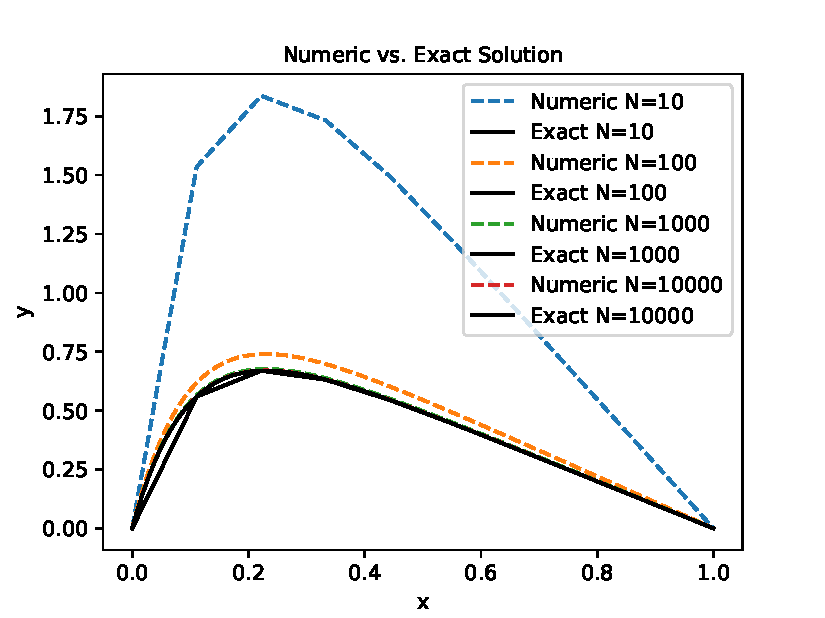
\includegraphics[scale=0.75]{Problem 7/Num.vs.Exact_Ns.pdf}%Imports the figure.
    \caption{Plot of Numeric vs. Exact solutions of x}
    \label{fig:Numeric vs. Exact Solution}
\end{figure}

\lstinputlisting[label= {listing3},language=C++]{Problem 7/prob7.cpp}
\begin{lstlisting}[label= {listing3},language=C++, caption=C++ program]
\end{lstlisting}

\lstinputlisting[label= {listing4},language=Python]{Problem 7/prob7.py}
\begin{lstlisting}[label= {listing4},language=Python, caption=Python plot script]
\end{lstlisting}

\subsection*{Problem VIII}
\subsubsection*{Problem VIII a.}
In this task we're to make a plot that shows the absolute error, by using equation(\ref{likn23}), if so we'll get this plot that shows us the absolute error as a function of $x_i$, and to show different choices $N$. 
\begin{figure}[h!]
    \centering
    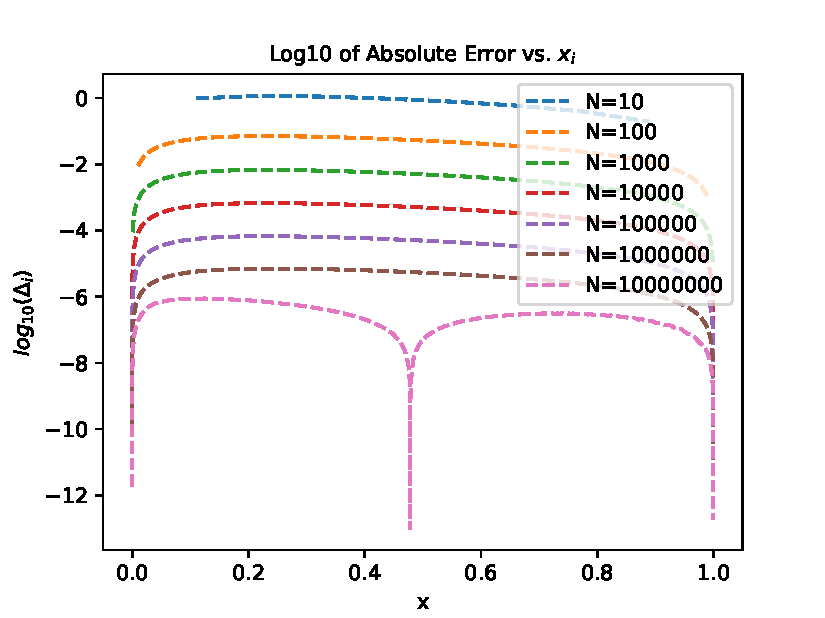
\includegraphics[width=3in]{Problem8/logAbsError_plot.pdf}
    \caption{$log_{10}(\Delta_i)$ as a function of $x_i$, for multiple choices of N}
    \label{fig2}
\end{figure}
\begin{equation}\label{likn23}
    log_{10}(\Delta_i)= log_{10}(|u_i-v_i|
\end{equation}


\subsubsection*{Problem VIII b.} And in this task we're to make the similarly plot of the relative error:
\begin{equation*}
    log_{10}(\epsilon_i)= log_{10}\Big|\frac{u_i-v_i}{u_i}\Big|
\end{equation*}
We'll have the following graph in figur(\ref{fig3}) that shows us the complete solution

\begin{figure}[h!]
    \centering
    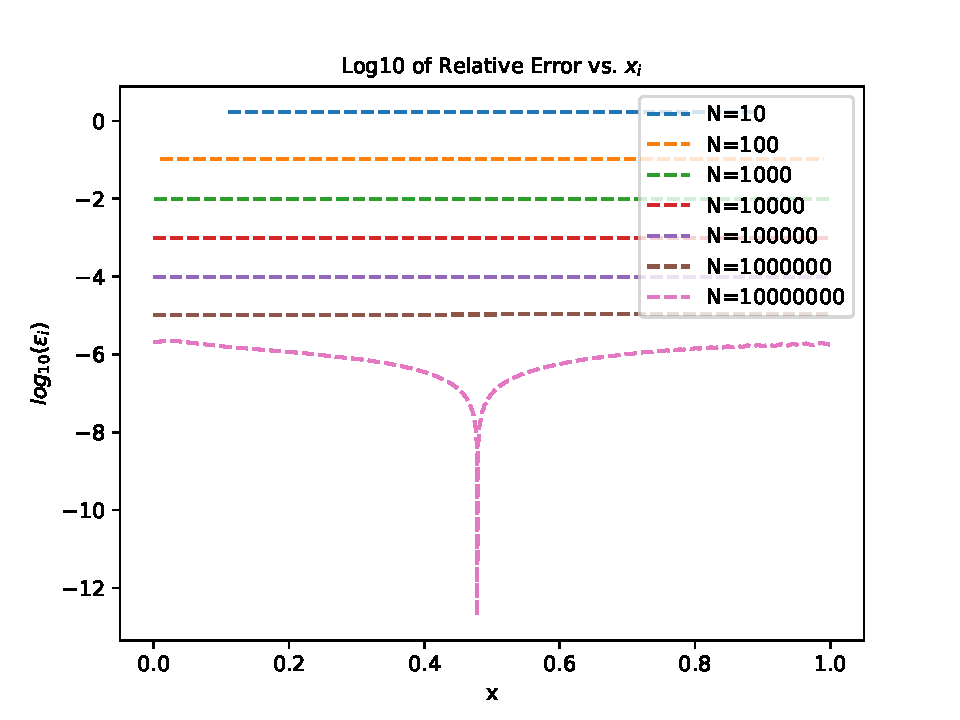
\includegraphics[width=3in]{Problem8/logRelError_plot.pdf}
    \caption{Relative error as a function of $x_i$ for N[10,10$^7$]}
    \label{fig3}
\end{figure}
\pagebreak
\subsubsection*{Problem VIII c.}
In this task we're to visualize the maximum relative error $max(\epsilon_i)$ for each choice of up to N = 10$^7$. 
\begin{figure}[h!]
    \centering
    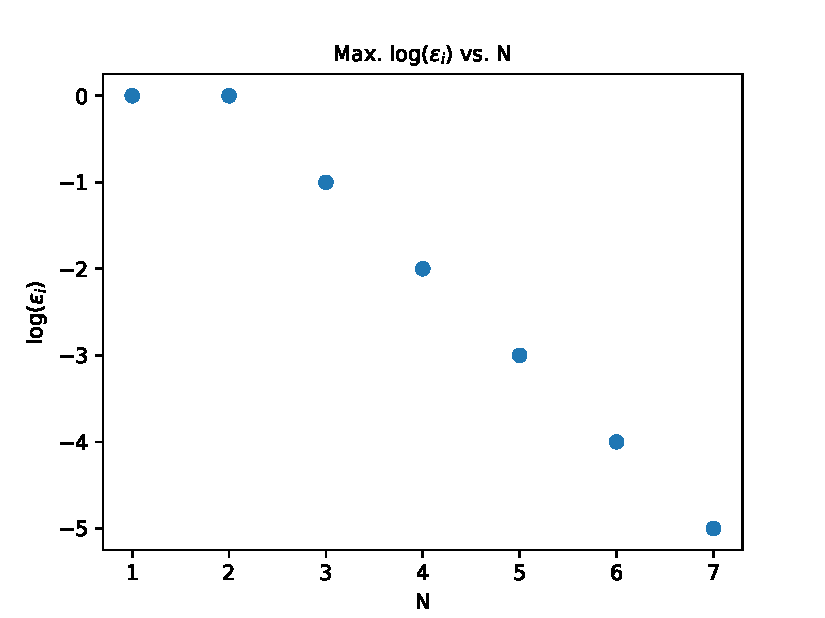
\includegraphics[width=3in]{Problem8/Log10Max_Relative_Error.pdf}
    \caption{Maximum realtive error as a function of N, as for N to each step from $10^1$ till $10^7$}
    \label{fig:my_label}
\end{figure}

For each choice of $n$ from $n$ = $10$ to $10^7$ the plots in \textit{Figure 5} show the corresponding maximum relative error. \\

Based on our results, we see that the higher value for the choice of $N$ is, the lower the value for absolute and relative error. Therefore, the more reliable the results of the approximation becomes. However, higher choice of $N$ also results in more data points to be evaluated resulting in unnecessary longer running time for the program.



\subsection*{Problem IX} 
Now we're to specialize our algorithm from problem  for our special case where \textbf{A} is specified by the signature $(-1, 2, -1)$, that is with 
\begin{equation*}
    \Vec{a}= [-1,-1,\hspace{0.00001cm}...\hspace{0.1cm},-1]\\
\end{equation*}
\begin{equation*}
    \Vec{b}= [\hspace{0.2cm}2,\hspace{0.2cm}2,\hspace{0.001cm}...\hspace{0.1cm},2\hspace{0.2cm}]\\
\end{equation*}
\begin{equation*}
    \Vec{c}= [-1,-1,\hspace{0.001cm}...\hspace{0.1cm},-1]\\
\end{equation*}
\subsubsection*{ProblemIX a. b.}
That gives us our matrix \textbf{A}:

\begin{equation*}
\begin{bmatrix}
    2 & -1 & 0 & 0     \\ 
    -1 & 2 & -1 & 0    \\ 
    0 & -1 & 2 & -1    \\ 
    0 & 0 & -1 & 2     \\ 
\end{bmatrix}
\begin{bmatrix}
    v_1 \\
    v_2 \\
    v_3 \\
    v_4 \\
\end{bmatrix}
= 
\begin{bmatrix}
    g_1 \\
    g_2 \\
    g_3 \\
    g_4 \\
\end{bmatrix}
\end{equation*}
We can use the same procedure as we used in Problem 6 to solve this matrix-vector equations. However, since we know the following main, sub- and superdiagonal elements, we can just simplify our algorithm and reduce the FLOPs, we'll have:

\begin{tcolorbox}
\textbf{New resulting algorithm}
\begin{equation*}
    \Tilde{b}_i = \frac{i+1}{i}
\end{equation*}
\begin{equation*}
    \Tilde{g}_i = g_i +\frac{1}{\Tilde{b}_1}\cdot \Tilde{g}_{i-1} 
\end{equation*}
\begin{equation*}
    v_N = \frac{\Tilde{g}_N}{\Tilde{b}_N} 
\end{equation*}
\begin{equation*}
    v_i= \frac{\Tilde{g}_i+v_{i+1}}{\Tilde{b}_i} 
\end{equation*}
\end{tcolorbox}
\begin{flushleft}
So that means that the total FLOPs is $7n$ due to that $\pm 1$ for a large  n is insignificant. That means that we'll have $7n$ FLOPs for our new algorithm.
\end{flushleft}

\subsubsection*{ProblemIX c.}

The code that implements this new special algorithm is shown below in \textit{Listing 5}. The difference between this new code vs. the previous one is on the lines where we defined $\Tilde{b_i}$, $\Tilde{g}_i$, $v_N$, $v_i$ and the fact that we do not need to define and create the vector arrays $\Vec{a}$, $\Vec{b}$, and $\Vec{c}$

\lstinputlisting[label= {listing6},language=C++]{Problem 9/prob9.cpp}
\begin{lstlisting}[label= {listing6},language=C++, caption=C++ Program for Special Algorithm]
\end{lstlisting}


\subsection*{Problem X}

We run timing tests on our general and special algorithm based code. In \textit{Listing 6}, we run both of the algorithms into a for loop to repeat the run for each choice of $N$ for reliable timing results. 

\lstinputlisting[label= {listing7},language=C++]{Problem 10/prob10.cpp}
\begin{lstlisting}[label= {listing7},language=C++, caption=C++ Program for Time Test]
\end{lstlisting}
%\pagebreak
Using a python script such as \textit{Listing 8}, we get a table showing the time results for both algorithms.

\lstinputlisting[label= {listing8},language=Python]{Problem 10/prob10.py}
\begin{lstlisting}[label= {listing8},language=Python, caption=Python table plot script]
\end{lstlisting}

\textit{Listing 7} prints out the averages of the time results for the repeated runs for each $N$ used. These results are shown below.

\begin{table}[!h]
    \begin{subtable}[c]{0.5\textwidth}
    \centering
        \begin{tabular}{c@{\hspace{1cm}} c}
        \hline
        N & $\log_{10}$(Time[s]) \\
        \hline
        $10^1$ & -5.43 \\
        $10^2$ & -4.65 \\
        $10^3$ & -3.81 \\
        $10^4$ & -2.78 \\
        $10^5$ & -1.76 \\
        $10^6$ & -0.82 \\
        \hline
        \end{tabular}
        \subcaption{General Algorithm}
    \end{subtable}
%
    \begin{subtable}[c]{0.5\textwidth}
    \centering
        \begin{tabular}{c@{\hspace{1cm}} c}
        \hline
        N & $\log_{10}$(Time[s]) \\
        \hline
        $10^1$ & -5.93 \\
        $10^2$ & -5.10 \\
        $10^3$ & -4.11 \\
        $10^4$ & -3.12 \\
        $10^5$ & -2.09 \\
        $10^6$ & -1.13 \\
        \hline
        \end{tabular}
        \subcaption{Special Algorithm}
    \end{subtable}
\caption{Time Results}
\end{table}

Based on \textit{Table 2}, we see that the run time used for the Special Algorithm is less than the one for the General Algorithm. \\

This means that the Special Algorithm runs faster. This is due to the fact that we have reduced the number of FLOPs in our Special Algorithm.


\subsection*{Problem XI}
In this case we're to solve our matrix equation using the general LU decomposition approach. For the decomposition step to be N = $10^5$ we expect the laptop to go slower. Since a floating point number has 8 bytes and we have a matrix that stores $N x N$ we'll have $8\cdot 10^10$ bytes. That requires a severe amount of memory.  
\end{document}
